% !Mode:: "TeX:UTF-8"
%!TEX program  = xelatex

% \documentclass{cumcmthesis}
\documentclass[withoutpreface,bwprint]{cumcmthesis} %去掉封面与编号页
% \documentclass{apmcmthesis}

\usepackage{url}
\title{}
\tihao{C}
\baominghao{apmcm24212413}
% \schoolname{XX大学}
% \membera{小米}
% \memberb{向左}
% \memberc{哈哈}
% \supervisor{老师}
% \yearinput{2017}
% \monthinput{08}
% \dayinput{22}
\usepackage{ctex}
\usepackage{setspace}
\usepackage{lipsum}
\usepackage{graphicx}%插入图片
\usepackage{cite}
\usepackage{hyperref}
\usepackage{tikz}
\usepackage{titlesec}
\usepackage{lastpage}
\usepackage{fancyhdr}
\begin{document}
% \pagestyle{fancy}
% \pagestyle{frontmatterstyle}
\pagestyle{fancy}
\fancyhf{}
\lhead{\small \team}
\bibliographystyle{plain}% 参考文献引用格式
 \maketitle
 \begin{abstract}
    The global pet industry is experiencing rapid expansion, primarily due to the rise in disposable income and the increasing preference for pets as companions. This paper delves into the mathematical modeling of the pet industry's growth and forecasting, with a particular emphasis on the Chinese market and international trends. Utilizing ARIMA, polynomial interpolation, and multiple linear regression, the study examines the Chinese pet industry's trajectory over the past five years and projects its future for the next three years. The research also encompasses global market trends and the influence of economic factors such as tariffs on the pet food sector. The findings offer strategic insights and guidance for sustainable growth within the pet industry.
% \uwave{关注我们的微信公众号}:
\begin{figure}[htbp]
	\centering
	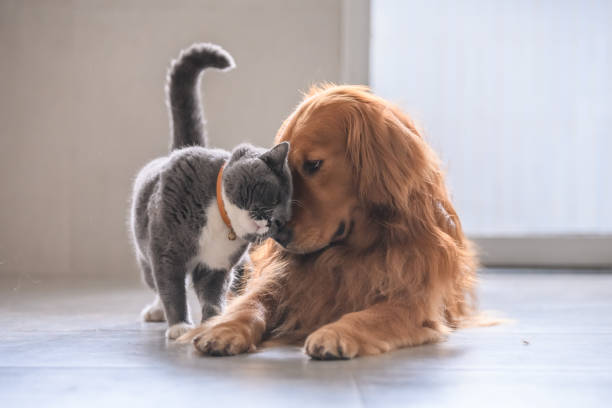
\includegraphics[scale=2.5]{istockphoto-992637094-612x612}
	\caption{British short hair cat and golden retriever stock photo\cite{1}}
\end{figure}
% \centerline{
\includegraphics[width=5cm]{gongzhonghao}}
% \caption{this is Ali}

\keywords{Pet Industry, Mathematical Models, ARIMA, Polynomial Interpolation, Multiple Linear Regression, Forecasting, Market Analysis, Economic Factors, Pet Food, Sustainable Development}
\end{abstract}
%目录
\tableofcontents
\setcounter{page}{1}
\rhead{\small  Page \thepage\ of 24}
\section{Problem Restatement}

This problem requires analyzing and forecasting the development trends of the pet industry in China and globally, with a focus on the pet food market. The analysis should combine historical data and additional data collected, building mathematical models for prediction. The specific tasks are as follows:
\subsection{Question 1: Development of China's Pet Industry}

\subsubsection{Objective}
Analyze the development of China's pet population over the past five years by different pet types.
\subsubsection{Factors}
Look into economic factors, societal trends, and market changes.
\subsubsection{Modeling Task}
Develop a mathematical model to predict the growth and development of China's pet population for the next three years.
\subsection{Question 2: Global Pet Industry Development}
\subsubsection{Objective}
Analyze the development of the global pet industry, focusing on different regions and pet types.
And predict the global demand for pet food over the next three years.
\subsubsection{Modeling Task}
Create a model to forecast the global demand for pet food over the next three years, based on data provided.
\subsection{Question 3: China's Pet Food Industry}
\subsubsection{Objective}
Analyze the development of China's pet food industry, specifically its production and export values.
\subsubsection{Modeling Task}
Predict China's pet food production and export trends over the next three years.
\subsection{Question 4: Impact of Foreign Economic Policies}
\subsubsection{Objective}
Analyze the impact of foreign economic policies on China's pet industry, focusing on trade barriers and tariffs.
\subsubsection{Modeling Task}
Develop a model to assess the impact of these policies on China's pet food industry and suggest strategies for sustainable development.
\section{Model Assumptions}

\begin{itemize}
    \item Stability of human society
    \item Exclusion of potential future policies related to pets
    \item Ignoring changes in pet population due to major incidents
\end{itemize}

\section{Symbol Explanation}
\begin{center}
\begin{tabular}{cc}
 \hline
 \makebox[0.3\textwidth][c]{Symbol}	&  \makebox[0.4\textwidth][c]{Meaning} \\ \hline
 $\ln$ 	    & Logarithmic Function \\ \hline
 $\sum$ 	    & Sum  \\ \hline
 $\prod$	    & Product  \\ \hline 
\end{tabular}
\end{center}

\section{Analysis}

\subsection{Question 1 Analysis}

The task first requires us to analyze the development trends of the pet industry in China by categorizing pets 
and identifying the factors that influence the growth of the pet industry.
We should begin by analyzing the data.
\subsubsection{Analyze factors}
\par The following data is provided to us in the problem.
\begin{table}[!htbp]
    \caption{2019-2023 Number of Pet Cats and Dogs in China (in 10,000s)} \centering
    \begin{tabular}{cccccc}
    \toprule[1.5pt]
    Pets/Years & 2023 & 2022 & 2021 & 2020 & 2019 \\
    \midrule[1pt]
    Cat & 6980 & 6536 & 5806 & 4862 & 4412 \\
    Dog & 5175 & 5119 & 5429 & 5222 & 5503 \\
    \bottomrule[1.5pt]
    \end{tabular}
    \end{table}
\par Plot the trend of changes in the pet population in China. 
A line chart is more intuitive than a table.
Thanks to the help of python, we can easily plot the line chart by the following code.
\begin{lstlisting}[language=python]
import pandas as pd
import matplotlib.pyplot as plt
with open('data_1.txt', 'r') as file:
    lines = file.readlines()
years = lines[0].split()[1:]
cat_data = lines[1].split()[1:]
dog_data = lines[2].split()[1:]
years = [int(year) for year in years]
cat_data = [int(num) for num in cat_data]
dog_data = [int(num) for num in dog_data]
plt.figure(figsize=(10, 6))
plt.plot(years, cat_data, marker='o', label='Cat')
plt.plot(years, dog_data, marker='o', label='Dog')
plt.xlabel('Year')
plt.ylabel('Number')
plt.title('Cat and Dog Numbers Over Years')
plt.legend()
plt.grid(True)
plt.show()
\end{lstlisting}
\begin{figure}[htbp]
	\centering
	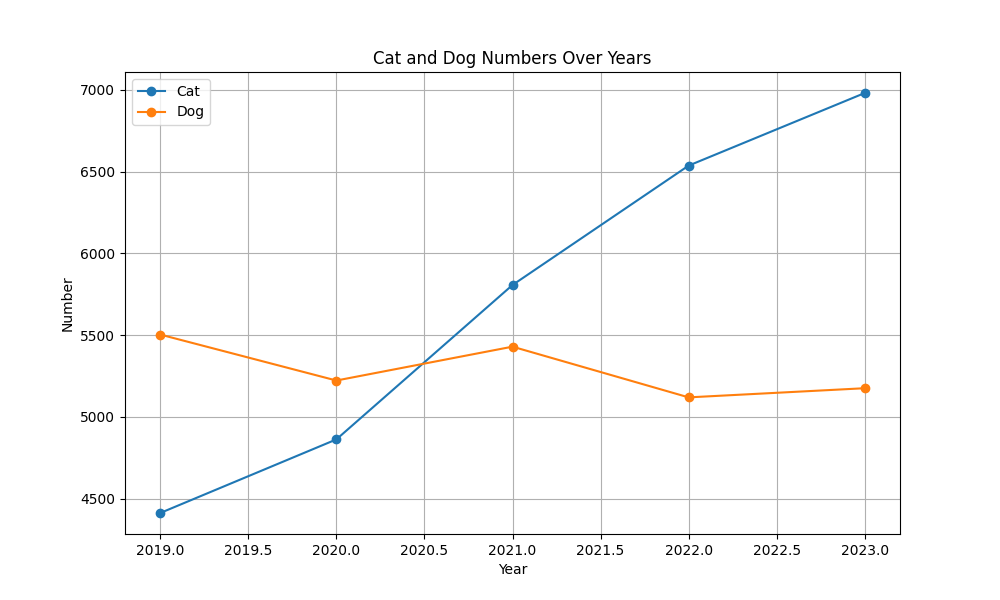
\includegraphics[scale=0.6]{Figure_2}
	\caption{Number of Cat and Dog in China from 2019 to 2023}
\end{figure}
\par From the graph, we can see that the number of cats is increasing, while the number of dogs remains almost unchanged. This growth in the cat population is likely due to the improvement in living standards, with more and more people beginning to keep pets.
Therefore, GDP is likely one of the factors influencing the pet population. By reviewing relevant data, we found a strong correlation between the growth rate of GDP and the growth rate of the pet population.
Thus, to predict the growth of the pet population, we can use the growth rate of GDP as an indicator.
As for dogs, we did not find a direct relationship between the GDP growth rate and the growth rate of the dog population. However, we can be certain that the development of the pet economy will drive the growth of the pet population.
Hence, the pet economy is likely to have a strong correlation with the growth of the pet population.
\par Summarizing the above analysis, we assume that the growth of the pet population is influenced by the growth rate of GDP.
\subsubsection{Polynomial Interpolation}
\par We aim to predict the data for the next three years based on the data from the previous five years, starting with polynomial interpolation.
\begin{definition}[Polynomial Interpolation]
Given \( n+1 \) points, polynomial interpolation refers to finding a polynomial such that it satisfies the condition
\[
    P(x) = a_n x^n + a_{n-1} x^{n-1} + \dots + a_1 x + a_0
\]
That is, the image of the polynomial \( y = P(x) \) must pass through the given \( n+1 \) points \( (x_i, y_i) \).
\end{definition}
\par Because \( P(x) \) can pass through these existing points and \( P(x) \) is a polynomial, \( P(x) \) may indeed reflect the trend of data changes to some extent.
\par We tried simple polynomial interpolation, with time as the independent variable and the number of cats and dogs as the dependent variable, to perform polynomial interpolation.
\begin{lstlisting}[language=python]
for n in range(1, 10):
    coeffs_cat = np.polyfit(years, cat_data, n)
    coeffs_dog = np.polyfit(years, dog_data, n)
    y_poly_pred_cat = np.polyval(coeffs_cat, years)
    y_poly_pred_dog = np.polyval(coeffs_dog, years)
    new_x = np.array([2019, 2020, 2021, 2022, 2023, 2024, 2025, 2026])
    new_y_cat = np.polyval(coeffs_cat, new_x)
    new_y_dog = np.polyval(coeffs_dog, new_x)
    plt.figure(figsize=(10, 6))
    plt.plot(years, cat_data, marker='o', label='Cat')
    plt.plot(years, dog_data, marker='o', label='Dog')
\end{lstlisting}
\par Define \( k \) as the degree of the polynomial, \( n \) as the number of points, when \( k \geqslant  n \), Function polyfit can be considered as(in fact not because of simplicity) using Lagrange interpolation to perform polynomial interpolation.
\begin{definition}[Lagrange Interpolation]
    Given a set of distinct nodes \( x_0, x_1, \dots, x_n \) and the corresponding function values \( y_0, y_1, \dots, y_n \), the Lagrange interpolation polynomial \( L(x) \) is the polynomial that interpolates these points, defined as:

    \[
    L(x) = \sum_{i=0}^{n} y_i \ell_i(x)
    \]
    
    where \( \ell_i(x) \) is the \( i \)-th Lagrange basis polynomial, defined as:
    
    \[
    \ell_i(x) = \prod_{\substack{0 \leq j \leq n \\ j \neq i}} \frac{x - x_j}{x_i - x_j}
    \]
    
    This polynomial satisfies: \( \ell_i(x_j) = \delta_{ij} \), where \( \delta_{ij} \) is the Kronecker delta, which is 1 when \( i = j \) and 0 otherwise.
    
\end{definition}
\par The following is the result of the polynomial interpolation.
\clearpage
\begin{figure}[htbp]
	\centering
	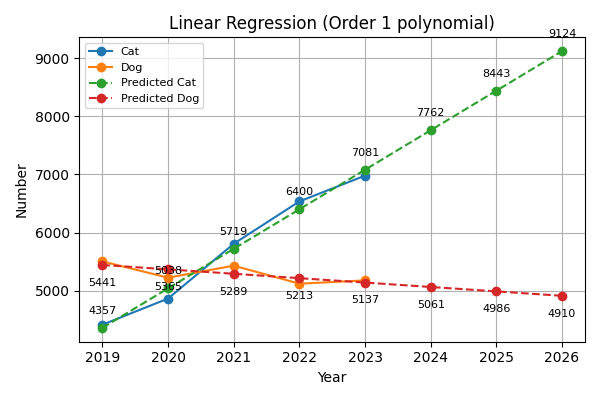
\includegraphics[scale=0.6]{q1_all1__}
	\caption{Linear Interpolation of Cat and Dog Numbers}
\end{figure}
\par We can find that although it is linear interpolation, the fitting effect is already very good.
However, when the degree of the polynomial is increased, the fitting effect is not significantly improved.
And because we only have five points, when the degree of the polynomial is greater than 5, the fitting effect is actually worse.
To solve the above problems and apply the two influencing factors mentioned earlier, we use the following model.
Its core idea is also fitting, but it is a higher dimension fitting.
Its essence has not changed, but the number of independent variables has increased.
\begin{figure}[htbp]
	\centering
	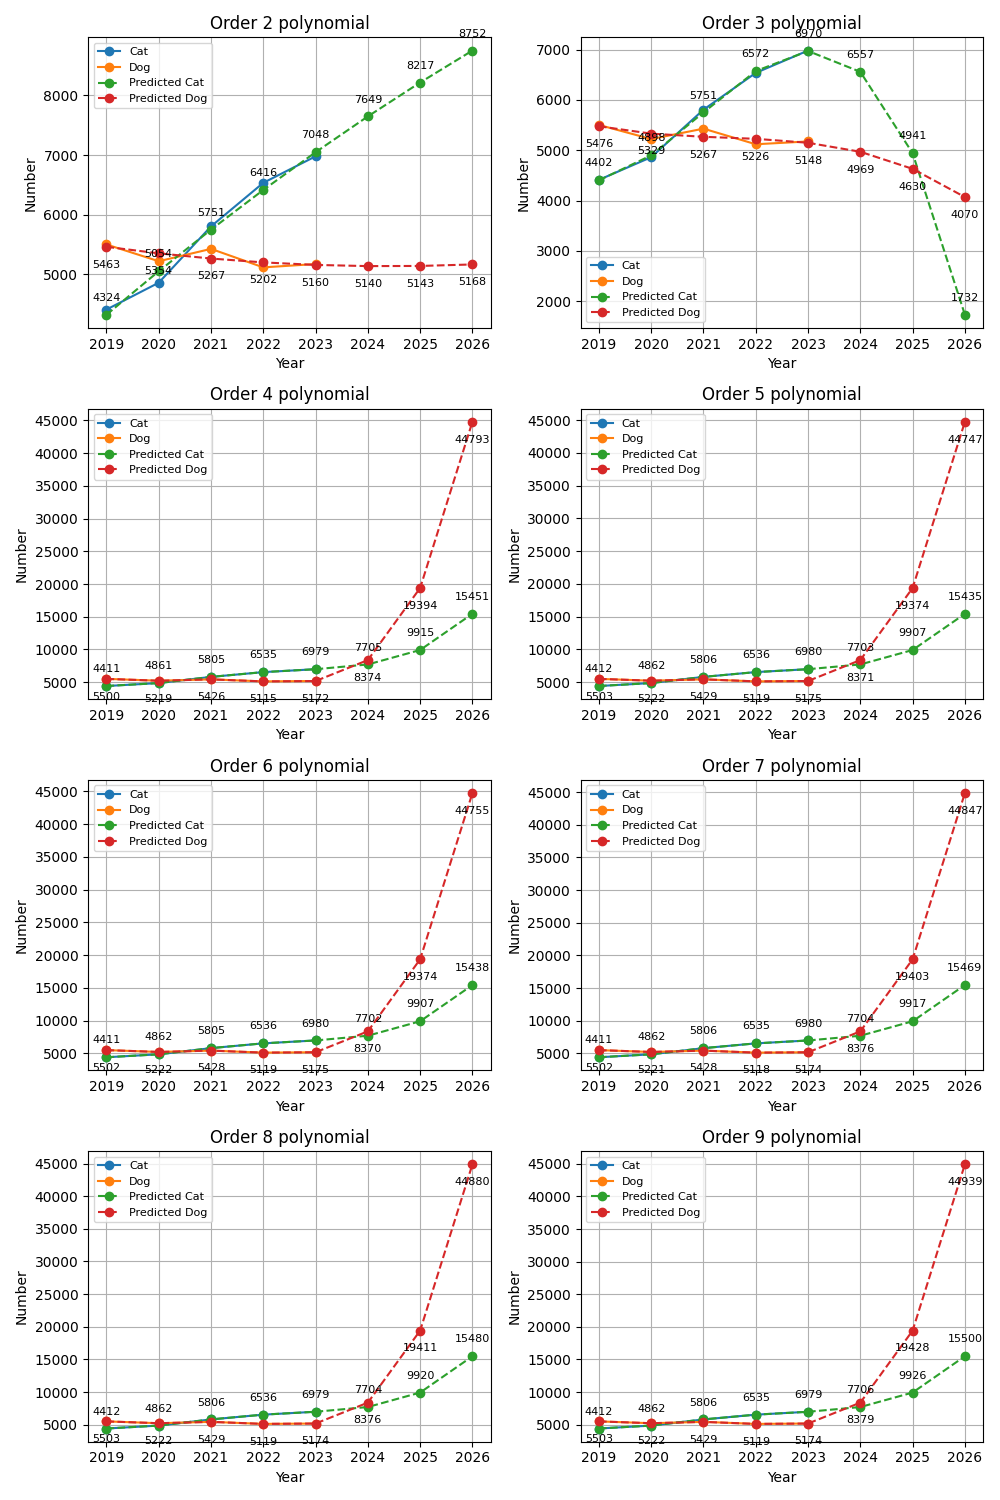
\includegraphics[width=.99\textwidth]{q1_all}
	\caption{Polynomial Interpolation of Cat and Dog Numbers}
\end{figure}
\subsubsection{Multiple Linear Regression and Logarithmic Curve Fitting}
\par First, we collected the relevant data.
\clearpage
% years 2023 2022 2021 2020 2019
% GDP 12614 12662 12617 10408 10143
\begin{table}[!htbp]
    \small
    \caption{2019-2023 GDP in China (in 10 billion yuan)\cite{2}} \centering
    \begin{tabular}{cccccc}
    \toprule[1.5pt]
    Years & 2023 & 2022 & 2021 & 2020 & 2019 \\
    \midrule[1pt]
    GDP & 12614 & 12662 & 12617 & 10408 & 10143 \\
    \bottomrule[1.5pt]
    \end{tabular}
\end{table}
% years 2023 2022 2021 2020 2019
% pet_industry_economy 3264 3069 2733 2259 2191
\begin{table}[!htbp]
    \small
    \caption{2019-2023 Pet Industry Economy in China (in 100 million yuan)\cite{3}} \centering
    \begin{tabular}{cccccc}
    \toprule[1.5pt]
    Years & 2023 & 2022 & 2021 & 2020 & 2019 \\
    \midrule[1pt]
    Pet Industry Economy & 3264 & 3069 & 2733 & 2259 & 2191 \\
    \bottomrule[1.5pt]
    \end{tabular}
\end{table}

\par Similarly, in three-dimensional space, we can also find a plane that fits all the points.
\begin{figure}[htbp]
	\centering
	\includegraphics[width=.85\textwidth]{figure_45}
	\caption{Three-Dimensional Linear Regression of Pet}
\end{figure}
\begin{definition}[Multiple Linear Regression]
Multiple Linear Regression is a statistical method used to model the relationship between two or more independent variables and a dependent variable. Suppose we have a dataset consisting of $n$ data points, each with $m$ independent variables and one dependent variable. The goal is to find the best-fitting hyperplane that describes the relationship between the independent and dependent variables.
\end{definition}

\begin{solution}
Assume we have $n$ observations, each with $m$ features. Each observation can be represented as:
\[
\mathbf{x}_i = (x_{i1}, x_{i2}, \dots, x_{im})^T, \quad y_i
\]
where $y_i$ is the dependent variable for the $i$-th observation, and $\mathbf{x}_i$ is the corresponding independent variable vector. Our goal is to fit the multiple linear regression model to the following equation:
\[
y_i = \beta_0 + \beta_1 x_{i1} + \beta_2 x_{i2} + \dots + \beta_m x_{im} + \epsilon_i
\]
where $\beta_0$ is the intercept term, $\beta_1, \beta_2, \dots, \beta_m$ are the regression coefficients, and $\epsilon_i$ is the error term, assumed to have zero mean and constant variance.


Let us represent all observations in matrix form. Suppose we have $n$ data points, each with $m$ features, the data can be written as:
\[
\mathbf{X} = \begin{pmatrix}
1 & x_{11} & x_{12} & \dots & x_{1m} \\
1 & x_{21} & x_{22} & \dots & x_{2m} \\
\vdots & \vdots & \vdots & \ddots & \vdots \\
1 & x_{n1} & x_{n2} & \dots & x_{nm}
\end{pmatrix}
\]
\[
\mathbf{y} = (y_1, y_2, \dots, y_n)^T
\]
where $\mathbf{X}$ is an $n \times (m+1)$ design matrix with the first column as ones, and $\mathbf{y}$ is an $n \times 1$ vector of the dependent variables.

The regression coefficients $\boldsymbol{\beta}$ are given by:
\[
\boldsymbol{\beta} = (\beta_0, \beta_1, \dots, \beta_m)^T
\]

Thus, the regression model in matrix form is:
\[
\mathbf{y} = \mathbf{X} \boldsymbol{\beta} + \boldsymbol{\epsilon}
\]
where $\boldsymbol{\epsilon}$ is the vector of errors.
To estimate the regression coefficients $\boldsymbol{\beta}$, we minimize the residual sum of squares (RSS):
\[
RSS = \sum_{i=1}^{n} (y_i - \hat{y}_i)^2 = (\mathbf{y} - \mathbf{X} \boldsymbol{\beta})^T (\mathbf{y} - \mathbf{X} \boldsymbol{\beta})
\]
Taking the derivative with respect to $\boldsymbol{\beta}$ and setting it equal to zero, we obtain the normal equation:
\[
\mathbf{X}^T \mathbf{X} \boldsymbol{\beta} = \mathbf{X}^T \mathbf{y}
\]
Solving this equation gives the estimated regression coefficients:
\[
\boldsymbol{\beta} = (\mathbf{X}^T \mathbf{X})^{-1} \mathbf{X}^T \mathbf{y}
\]
\end{solution}
\begin{lstlisting}[language=python]
# key code
from sklearn.linear_model import LinearRegression
regressor_cat = LinearRegression()
regressor_cat.fit(X_cat, cat)
x_grid, y_grid = np.meshgrid(np.linspace(x.min(), x.max(), 30),
                                np.linspace(y.min(), y.max(), 30))
z_pred_cat = regressor_cat.predict(np.column_stack(
    (x_grid.ravel(), y_grid.ravel()))).reshape(x_grid.shape)
surf_cat = ax.plot_surface(
    x_grid, y_grid, z_pred_cat, alpha=0.3, cmap='Reds')
\end{lstlisting}
\par the problem is that we only have one independent variable, which is time,
and only one dimension of data, so we can't find the corresponding points on the plane.
we have to predict the data of GDP and pet industry economy 
so as to find the corresponding points on the plane.
One good way is to use the linear regression model.
\begin{figure}[htbp]
	\centering
	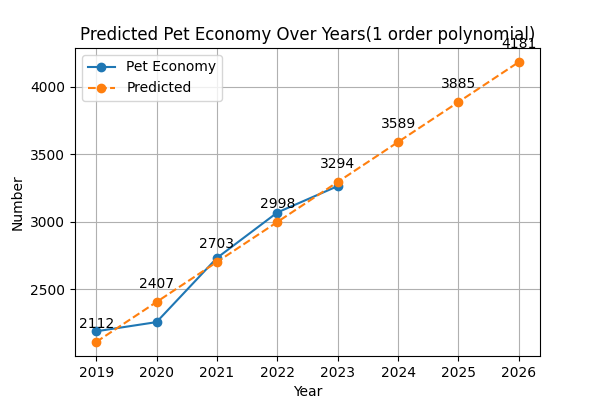
\includegraphics[width=.6\textwidth]{q3_1_}
	\caption{Linear Regression of Pet Industry Economy-Year-Pets}
\end{figure}
\begin{figure}[htbp]
	\centering
	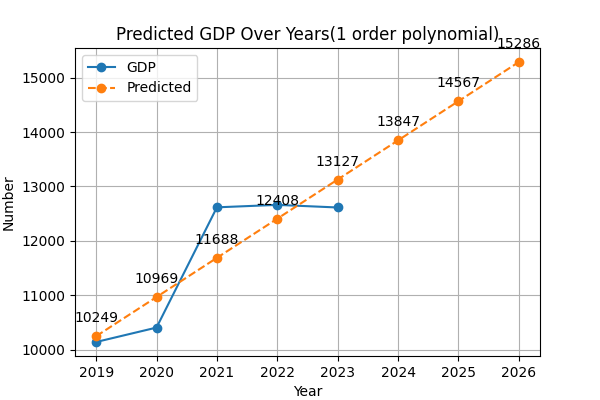
\includegraphics[width=.6\textwidth]{q2_1_}
	\caption{Linear Regression of GDP-Year-Pets}
\end{figure}
\par We can see that the fitting effect is very good for pet industry economy.
But as for GDP, the fitting effect is a bit poor. It original data looks like a logarithm curve.
Using logarithm curve to fit the data, we can get a better fitting effect.
\begin{definition}[Logarithmic Curve Fitting]
The logarithmic model is expressed as:
\[
y = \sum_{i=0}^{n} a_i [\ln(bx + c)]^i = a_0 + a_1 \ln(bx + c) + a_2 [\ln(bx + c)]^2 + \dots + a_n [\ln(bx + c)]^n
\]
where \(a_i\), \(b\), and \(c\) are constants, and \(x\) and \(y\) are the data points.
\end{definition}
\begin{solution}
To fit the logarithmic curve, we can use the following procedure.
let \(z = \ln(bx + c)\), then the model becomes:
\[
y = \sum_{i=0}^{n} a_i z^i = a_0 + a_1 z + a_2 z^2 + \dots + a_n z^n
\]
which is a polynomial model, we can use the polynomial regression model to fit the data.
\end{solution}
\begin{figure}[htbp]
	\centering
	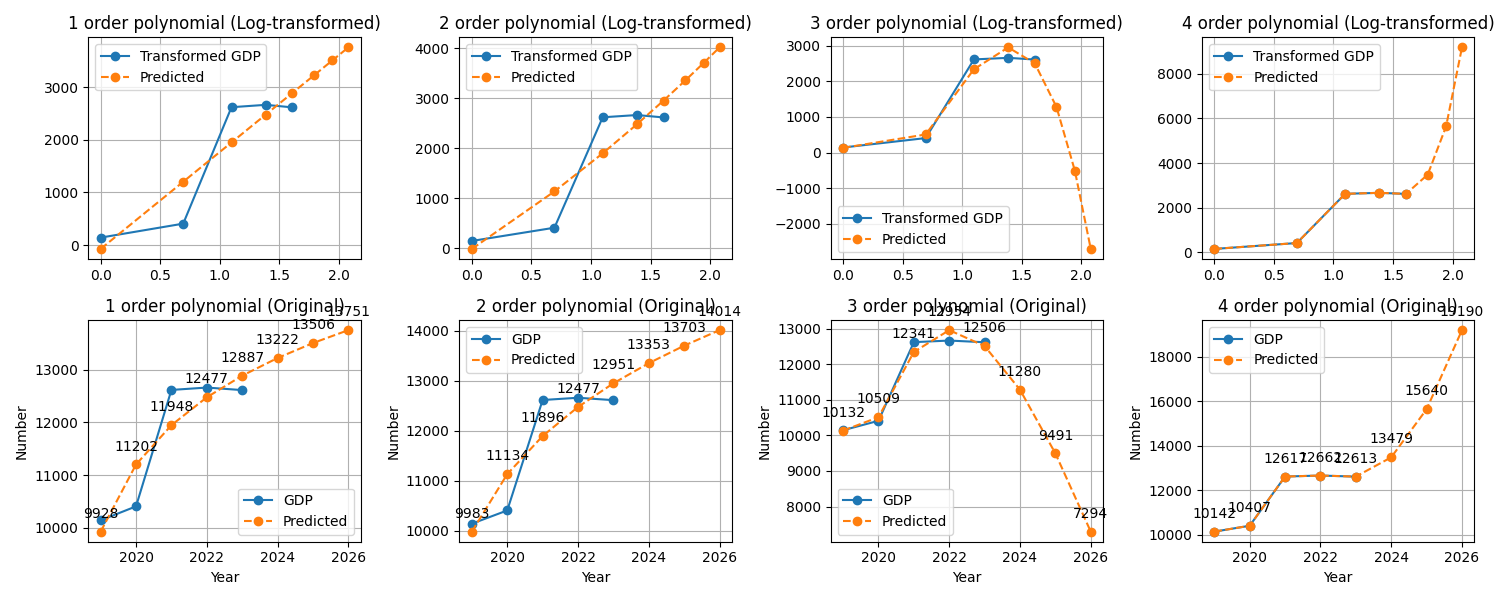
\includegraphics[width=.99\textwidth]{qlog_all}
	\caption{Logarithmic Curve Fitting of GDP}
\end{figure}
\par We choose the 4th order polynomial to fit the data.
The reason is that China's GDP grows faster and faster despite the overfitting.
\par So we get predicted pet industry economy and GDP data.

\begin{table}[!htbp]
    \small
    \caption{2019-2026 Predicted Pet Industry Economy(in 100 million yuan) and GDP(in 10 billion yuan) in China} \centering
    \begin{tabular}{ccccccccc}
    \toprule[1.5pt]
    Years & 2026 & 2025 & 2024 & 2023 & 2022 & 2021 & 2020 & 2019 \\
    \midrule[1pt]
    Pet Industry Economy & 4181 & 3885 & 3589 & 3294 & 2998 & 2703 & 2407 & 2112 \\
    GDP & 19190 & 15640 & 13479 & 12614 & 12662 & 12617 & 10408 & 10143 \\
    \bottomrule[1.5pt]
    \end{tabular}
\end{table}
\par Applying the two factors to the multiple linear regression model,
we can get the predicted pet population.
\clearpage
\begin{figure}[htbp]
	\centering
	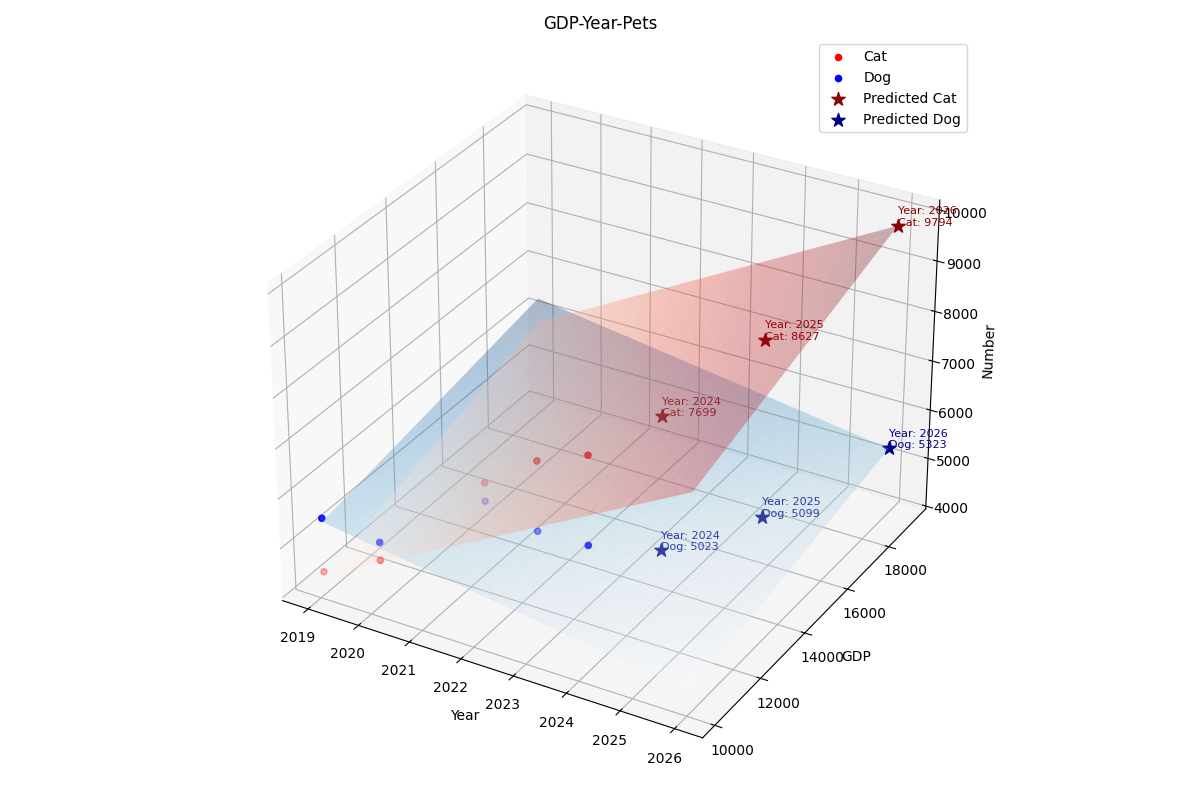
\includegraphics[width=.99\textwidth]{Figure_11}
	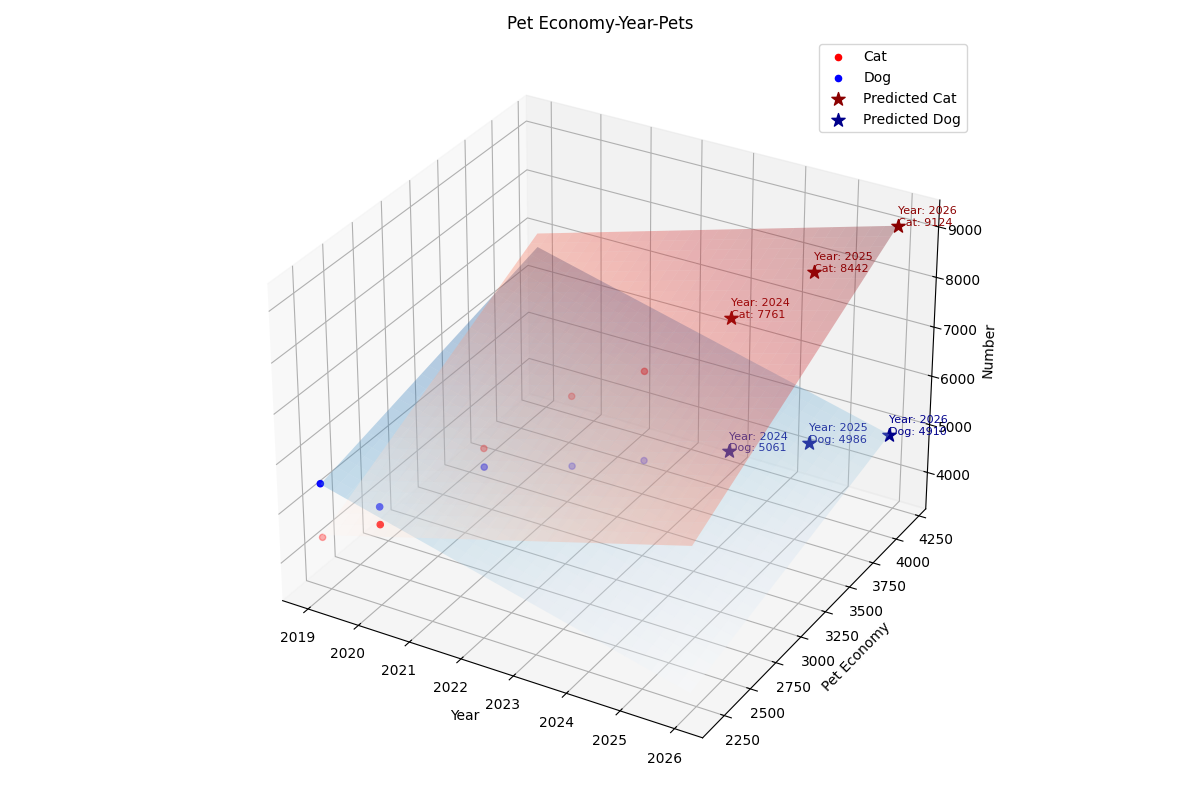
\includegraphics[width=.99\textwidth]{Figure_12}
	\caption{Predicted Pet Population in China}
\end{figure}
\clearpage
\par Combine the two factors, we use 4 dimension multiple linear regression model to fit the data.
\begin{figure}[htbp]
	\centering
	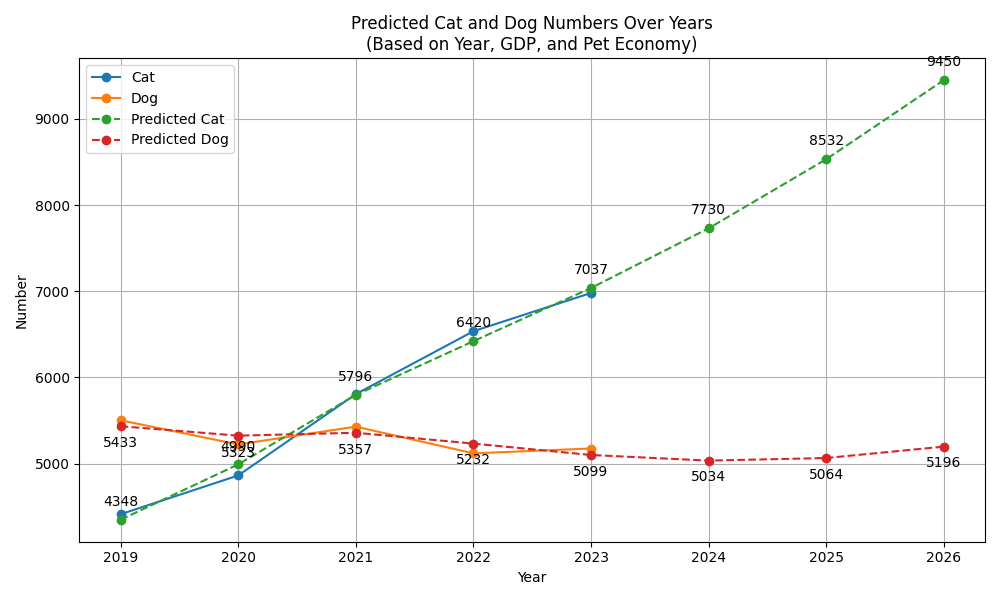
\includegraphics[width=.99\textwidth]{Figure_13}
	\caption{Predicted Pet Population in China based on GDP and Pet Industry Economy}
\end{figure}
\begin{table}[!htbp]
    \small
    \caption{2019-2026 Predicted Pet Population in China (in 10000s)} \centering
    \begin{tabular}{ccccccccc}
    \toprule[1.5pt]
    Years & 2026 & 2025 & 2024 & 2023 & 2022 & 2021 & 2020 & 2019 \\
    \midrule[1pt]
    Cat & 9450 & 8532 & 7730 & 6980 & 6536 & 5806 & 4862 & 4412 \\
    Dog & 5196 & 5064 & 5034 & 5175 & 5119 & 5429 & 5222 & 5503 \\
    \bottomrule[1.5pt]
    \end{tabular}
\end{table}
\subsection{Question 2 Analysis}
\usetikzlibrary{positioning}
\begin{figure}[htbp]
    \centering
    \begin{tikzpicture}[
        node distance=1.5cm,
        box/.style={rectangle,draw,rounded corners,minimum width=2cm,minimum height=0.8cm},
        arrow/.style={->,>=stealth,thick}
    ]
        \node[box] (food) {Food Demand};
        \node[box,right=3cm of food] (pets) {Pet Population};
        \node[box,above right=0.4cm and 3cm of pets] (country) {Countries};
        \node[box,below right=0.4cm and 3cm of pets] (type) {Pet Types};
        
        \draw[arrow] (food) -- node[above,font=\small] {Positive Correlation} (pets);
        \draw[arrow] (pets) -- (country);
        \draw[arrow] (pets) -- (type);
    \end{tikzpicture}
    \caption{Pet Food Demand Analysis Chain}
\end{figure}
\begin{assumption}
    The demand for pet food of the same type of pet is the same in different countries.
\end{assumption}
 \[demands=\sum_{i=1}^{n} demand_i=\sum_{i=1}^{k} count_i \times demand_{pet_i}\]
\par To analyze the development of the global pet industry by pet type and country,
we first analyze the given data.
\begin{figure}[htbp]
	\centering
	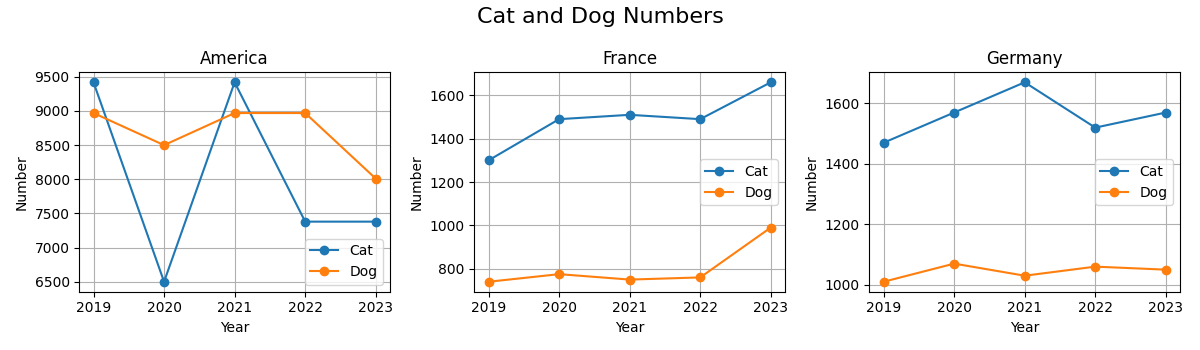
\includegraphics[width=.99\textwidth]{all_countries_pets.png}
	\caption{Cat and Dog Numbers Over Years by Country}
\end{figure}
\begin{figure}[htbp]
	\centering
	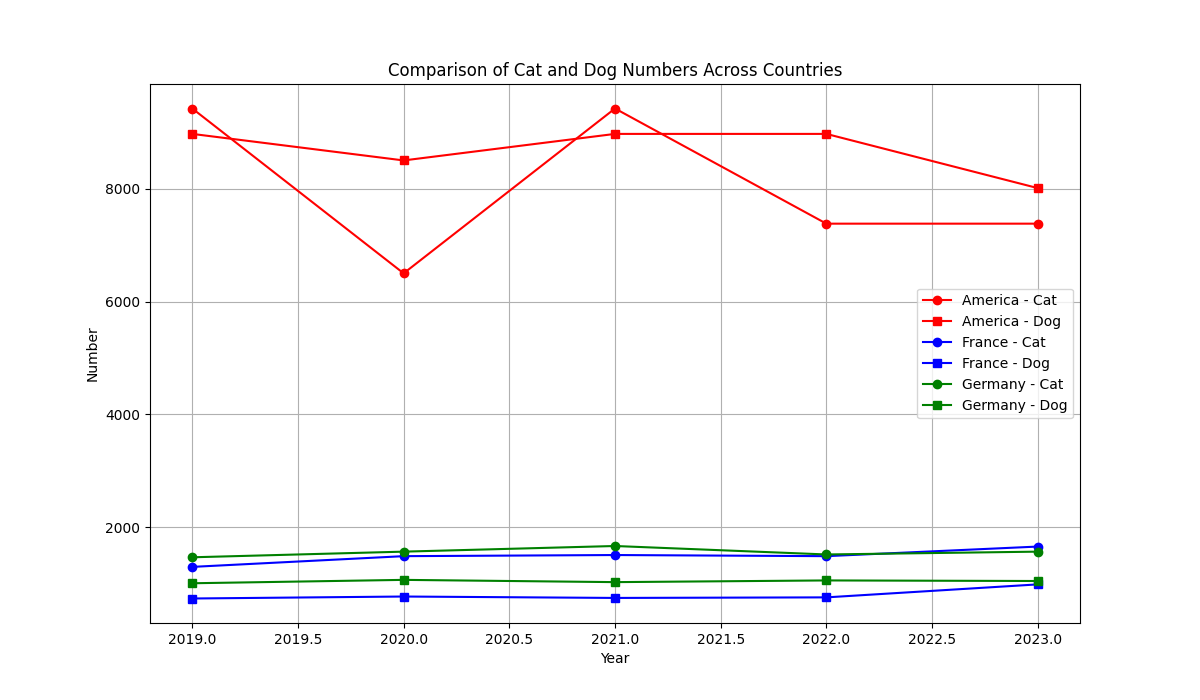
\includegraphics[width=.7\textwidth]{combined_pets.png}
	\caption{Cat and Dog Numbers Over Years by Country}
\end{figure}
\par We can see that the number of cats and dogs in America is much larger than that in France and Germany.
and the number of cat and dog is almost the same.
\par We aim to forecast the global demand for pet food in the next three years.
Because the pet food market is closely related to the pet population, we can use the predicted pet population to forecast the demand for pet food.
For dataset that is time series, we can use the ARIMA model to forecast the data.

\subsubsection{Forecast Population and ARIMA}
\begin{definition}[ARIMA Model]
The ARIMA model, which stands for AutoRegressive Integrated Moving Average, is a popular method for forecasting time series data. It is particularly useful for predicting future points in a series based on its past values. The ARIMA model is defined by three parameters:
\[
ARIMA(p, d, q)
\]
where:
\begin{itemize}
    \item \( p \) is the order of the autoregressive (AR) part.
    \item \( d \) is the degree of differencing required to make the time series stationary.
    \item \( q \) is the order of the moving average (MA) part.
\end{itemize}

The AR part of the model represents a regression of the current value on its previous values. The general form for an autoregressive process of order \( p \) is:
\[
X_t = \phi_1 X_{t-1} + \phi_2 X_{t-2} + \cdots + \phi_p X_{t-p} + \epsilon_t
\]
where \( \phi_1, \phi_2, \dots, \phi_p \) are parameters, and \( \epsilon_t \) is white noise.

Differencing is applied to the time series to make it stationary. If the series is not stationary, we subtract the current value from the previous value, and repeat this process \( d \) times. The differenced series is:
\[
\Delta^d X_t = (1 - B)^d X_t
\]
where \( B \) is the backshift operator, i.e., \( B^k X_t = X_{t-k} \).

The MA part models the relationship between an observation and a residual error from a moving average model applied to lagged observations. A moving average process of order \( q \) is given by:
\[
X_t = \mu + \epsilon_t + \theta_1 \epsilon_{t-1} + \theta_2 \epsilon_{t-2} + \cdots + \theta_q \epsilon_{t-q}
\]
where \( \mu \) is the mean, \( \epsilon_t \) are the white noise errors, and \( \theta_1, \theta_2, \dots, \theta_q \) are the parameters.

Combining all the components, the ARIMA model for a time series \( X_t \) is:
\[
X_t = \mu + \phi_1 X_{t-1} + \cdots + \phi_p X_{t-p} + \epsilon_t + \theta_1 \epsilon_{t-1} + \cdots + \theta_q \epsilon_{t-q}
\]
where \( \mu \) is the mean, and the parameters \( \phi_i \) and \( \theta_j \) need to be estimated.
\end{definition}

\begin{lstlisting}[language=python]
# key code
from statsmodels.tsa.arima.model import ARIMA
cat_model = ARIMA(cat_data_array, order=(1, 1, 1))
cat_fit = cat_model.fit()
cat_pred = cat_fit.get_prediction(start=1, end=len(all_years)-1)
cat_predicted = np.concatenate(
    ([cat_data[0]], cat_pred.predicted_mean[:len(years)-1]))
cat_forecast = cat_pred.predicted_mean[len(years)-1:]
cat_all_data = np.concatenate((cat_predicted, cat_forecast))
\end{lstlisting}

%check table
\begin{table}[htbp]
% \small % 缩小表格字体
\tiny
\centering
\caption{ADF and Ljung-Box Test Results}
\begin{tabular}{llcccc}
\toprule
Country & Diff Order & Data Type & ADF Test & P-value & Stationarity/White Noise \\
\midrule
\multirow{4}{*}{America} & \multirow{4}{*}{0} & Cat(ADF) & 0.2371 & 0.7574 & Non-stationary \\
& & Dog(ADF) & 0.6919 & 0.8653 & Non-stationary \\
& & Cat(L-B) & 3.9598 & 0.0466 & Non-white noise \\
& & Dog(L-B) & 0.7603 & 0.3832 & White noise \\
\midrule
\multirow{4}{*}{America} & \multirow{4}{*}{1} & Cat(ADF) & 0.0000 & 0.6843 & Non-stationary \\
& & Dog(ADF) & 0.0000 & 0.6843 & Non-stationary \\
& & Cat(L-B) & 4.0165 & 0.0451 & Non-white noise \\
& & Dog(L-B) & 0.1711 & 0.6791 & White noise \\
\midrule
\multirow{3}{*}{America} & \multirow{3}{*}{2} & Cat(ADF) & -5.3474 & 0.0000 & Stationary \\
& & Dog(ADF) & -1.0087 & 0.2846 & Non-stationary \\
& & L-B Test & \multicolumn{3}{c}{Insufficient sample size} \\
\midrule
\multirow{4}{*}{France} & \multirow{4}{*}{0} & Cat(ADF) & -1.7786 & 0.0716 & Non-stationary \\
& & Dog(ADF) & -1.4080 & 0.1483 & Non-stationary \\
& & Cat(L-B) & 0.0000 & 1.0000 & White noise \\
& & Dog(L-B) & 0.0281 & 0.8669 & White noise \\
\midrule
\multirow{4}{*}{France} & \multirow{4}{*}{1} & Cat(ADF) & 0.0000 & 0.6843 & Non-stationary \\
& & Dog(ADF) & -0.0000 & 0.6843 & Non-stationary \\
& & Cat(L-B) & 0.4705 & 0.4928 & White noise \\
& & Dog(L-B) & 0.0167 & 0.8971 & White noise \\
\midrule
\multirow{3}{*}{France} & \multirow{3}{*}{2} & Cat(ADF) & -1.1357 & 0.2329 & Non-stationary \\
& & Dog(ADF) & -3.0520 & 0.0023 & Stationary \\
& & L-B Test & \multicolumn{3}{c}{Insufficient sample size} \\
\midrule
\multirow{4}{*}{Germany} & \multirow{4}{*}{0} & Cat(ADF) & -0.4659 & 0.5101 & Non-stationary \\
& & Dog(ADF) & -1.1406 & 0.2311 & Non-stationary \\
& & Cat(L-B) & 0.3825 & 0.5362 & White noise \\
& & Dog(L-B) & 3.0780 & 0.0794 & White noise \\
\midrule
\multirow{4}{*}{Germany} & \multirow{4}{*}{1} & Cat(ADF) & 0.0000 & 0.6843 & Non-stationary \\
& & Dog(ADF) & -0.0000 & 0.6843 & Non-stationary \\
& & Cat(L-B) & 0.6246 & 0.4294 & White noise \\
& & Dog(L-B) & 3.6171 & 0.0572 & White noise \\
\midrule
\multirow{3}{*}{Germany} & \multirow{3}{*}{2} & Cat(ADF) & -2.4400 & 0.0142 & Stationary \\
& & Dog(ADF) & -18.1111 & 0.0000 & Stationary \\
& & L-B Test & \multicolumn{3}{c}{Insufficient sample size} \\
\bottomrule
\end{tabular}
\end{table}
\par We can find that most of them are not stationary, but due to the small amount of data, the confidence of the results is not high.
We can still try to use the ARIMA model to predict the data.
Starting with (1,1,1) for all countries, we can get the predicted data.
\clearpage
\begin{figure}[htbp]
	\centering
	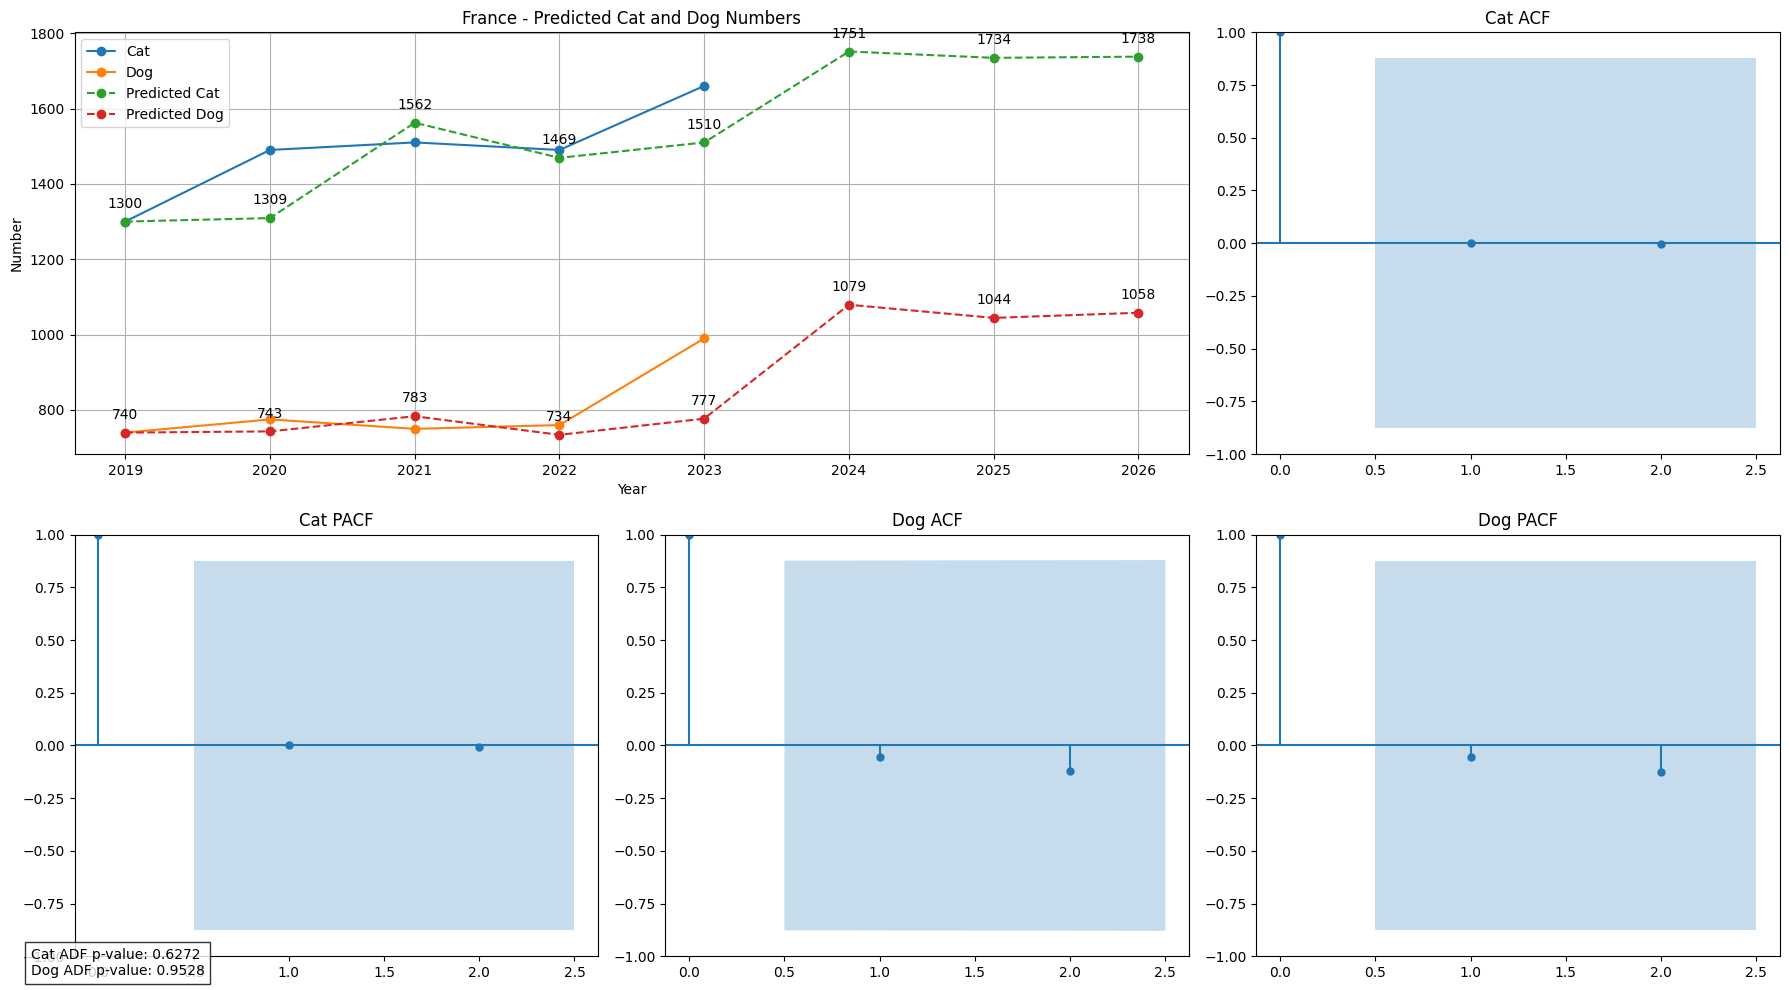
\includegraphics[width=.99\textwidth]{france_pets_forecast.png}
	\caption{Predicted Cat and Dog Population in France}
\end{figure}
\begin{figure}[htbp]
	\centering
	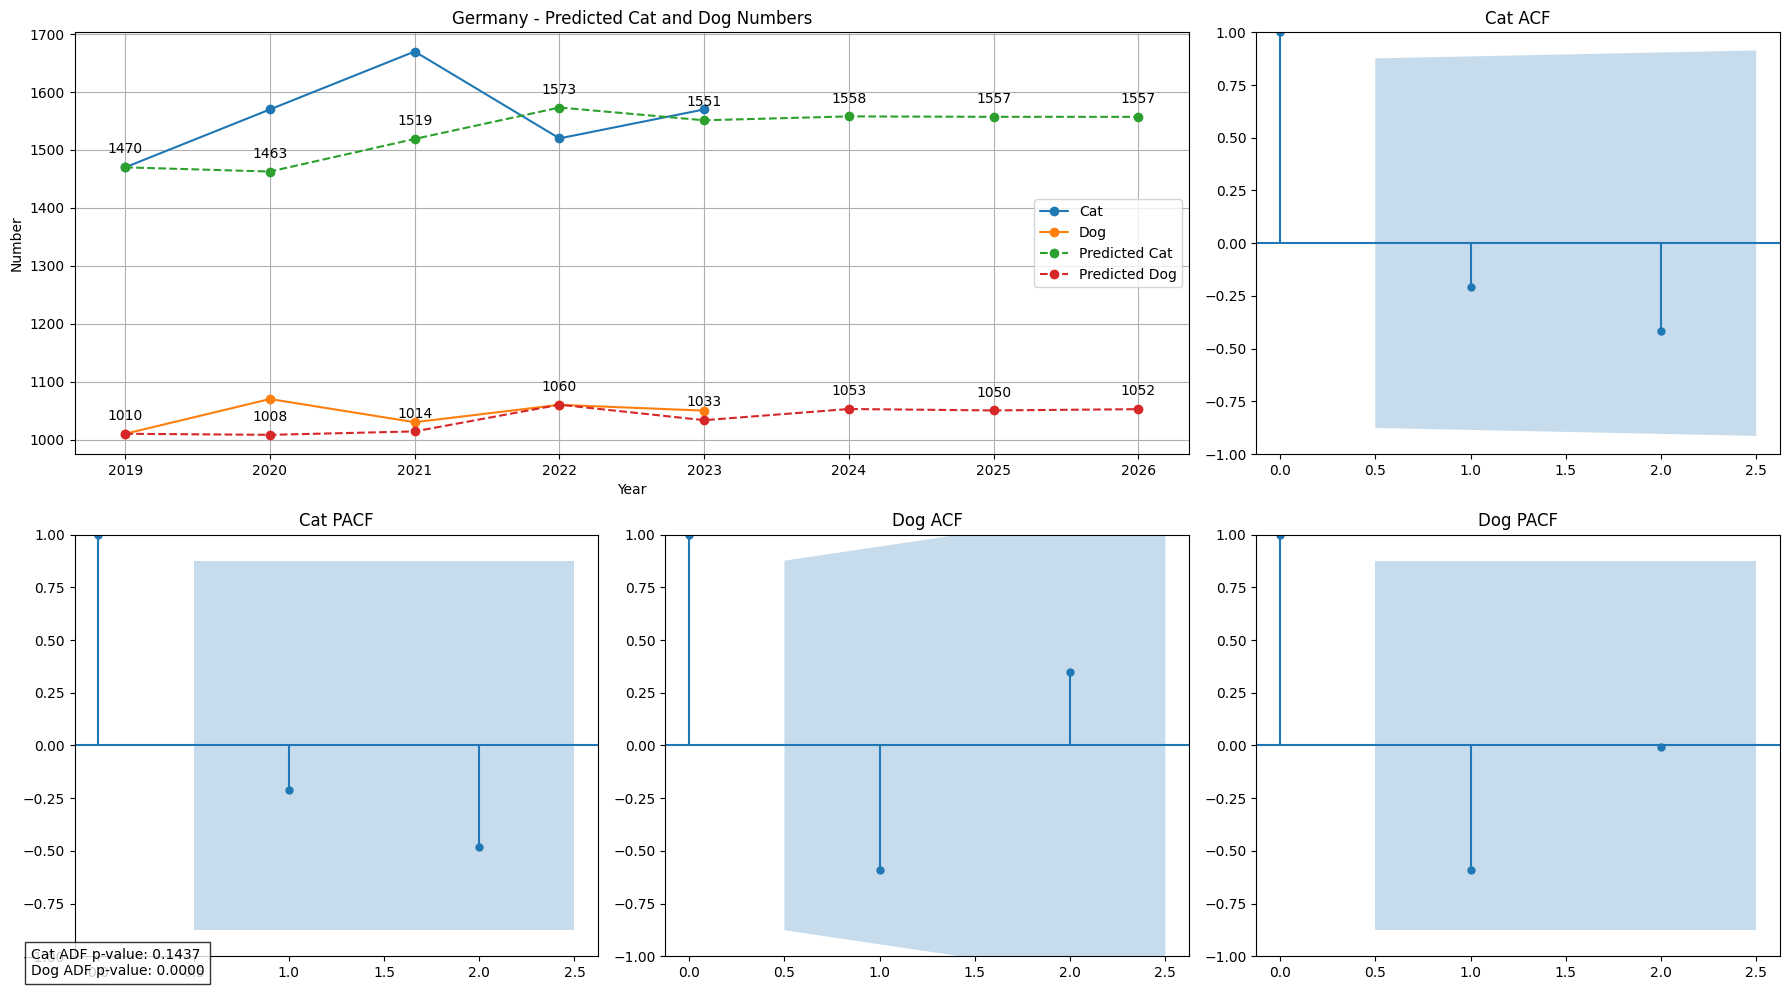
\includegraphics[width=.99\textwidth]{germany_pets_forecast.png}
	\caption{Predicted Cat and Dog Population in Germany}
\end{figure}
\par Beacause of the nearly stationary, France and Germany have a good fitting effect, we can use the predicted data to forecast the demand for pet food.

\clearpage
\begin{figure}[htbp]
	\centering
	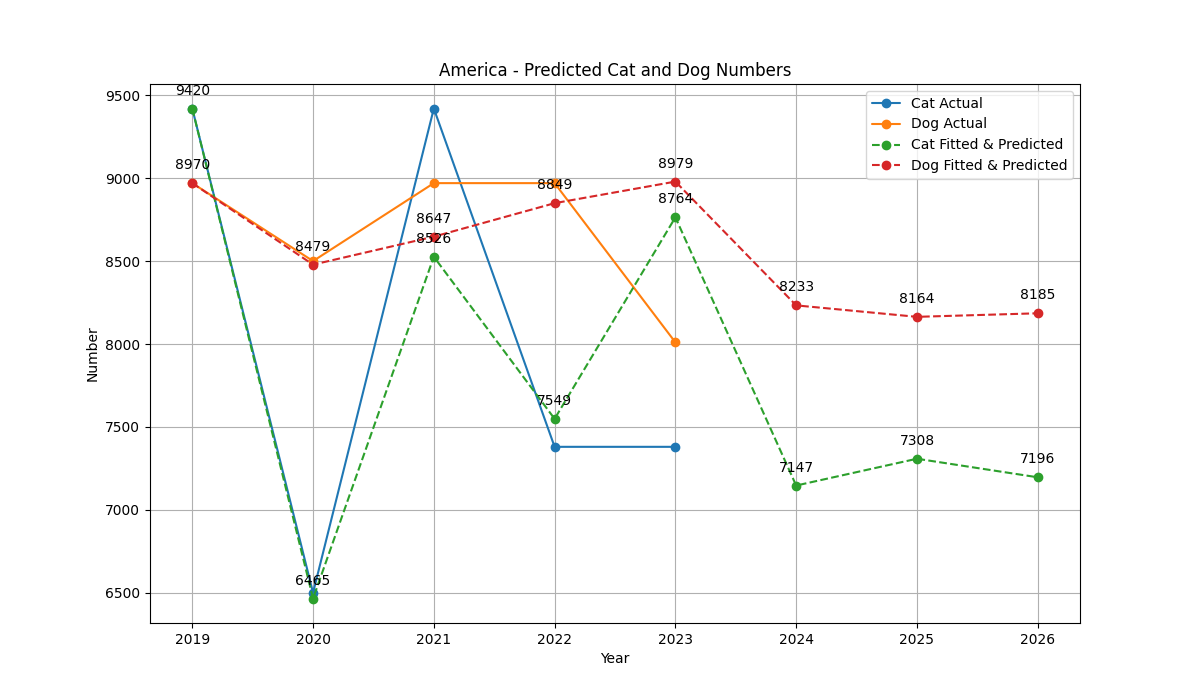
\includegraphics[width=.99\textwidth]{america_pets_forecast.png}
	\caption{Predicted Cat and Dog Population in America (poor fitting effect)}
\end{figure}
\par However, for America, because of the non-stationary, the fitting effect is not good. 
So we try to use the (1,k,1) model to fit the data.
And calculate the MSE of the fitting effect to find the best \(k\).
\begin{figure}[htbp]
	\centering
	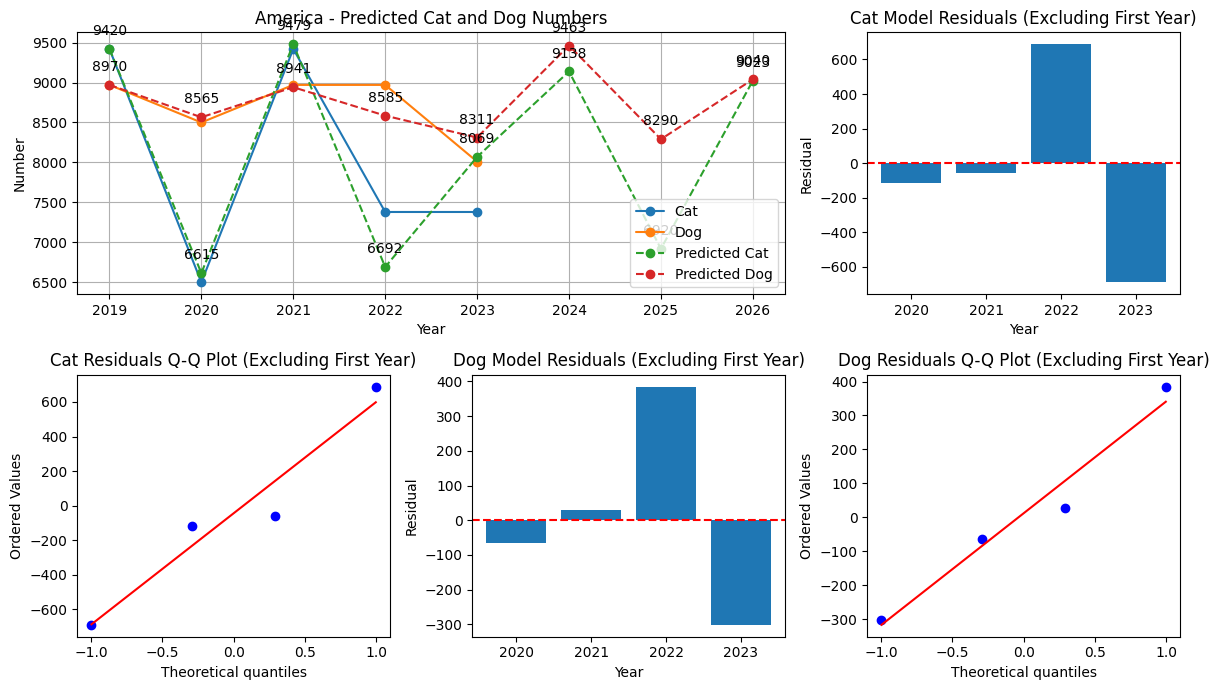
\includegraphics[width=.8\textwidth]{america_pets_forecast_k0.png}
	\caption{Predicted Cat and Dog Population in America (k=0)}
\end{figure}
\clearpage
\begin{figure}[htbp]
	\centering
	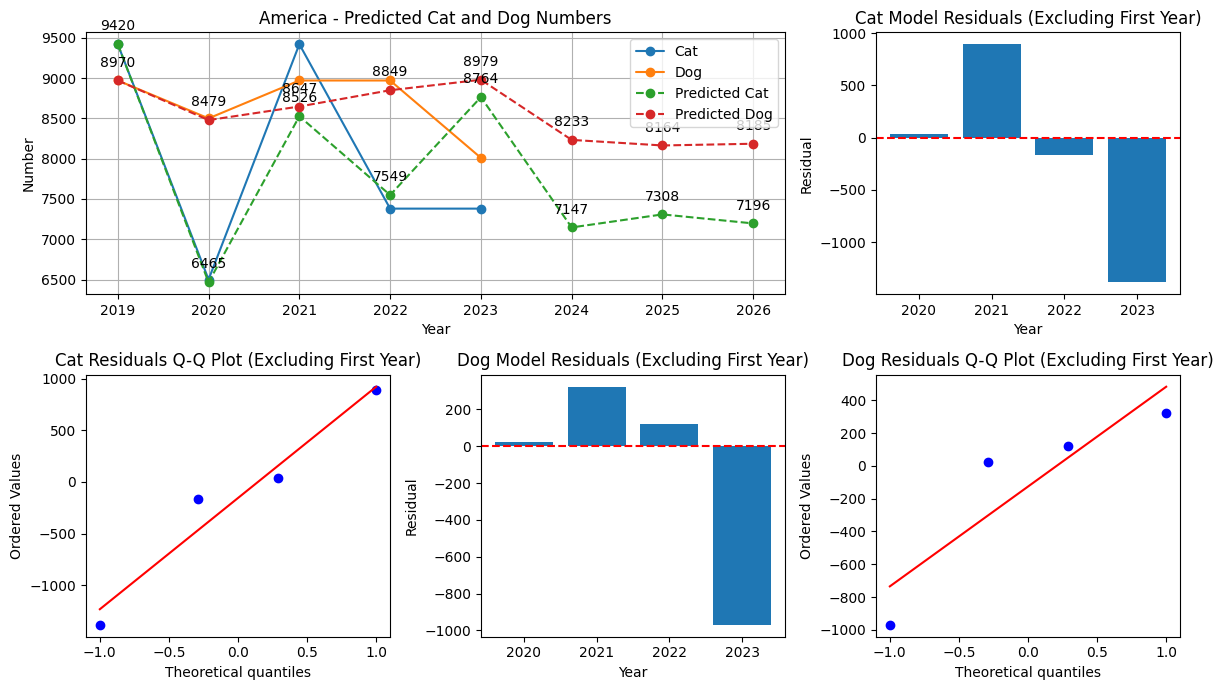
\includegraphics[width=.8\textwidth]{america_pets_forecast_k1.png}
	\caption{Predicted Cat and Dog Population in America (k=1)}
\end{figure}
\begin{figure}[htbp]
	\centering
	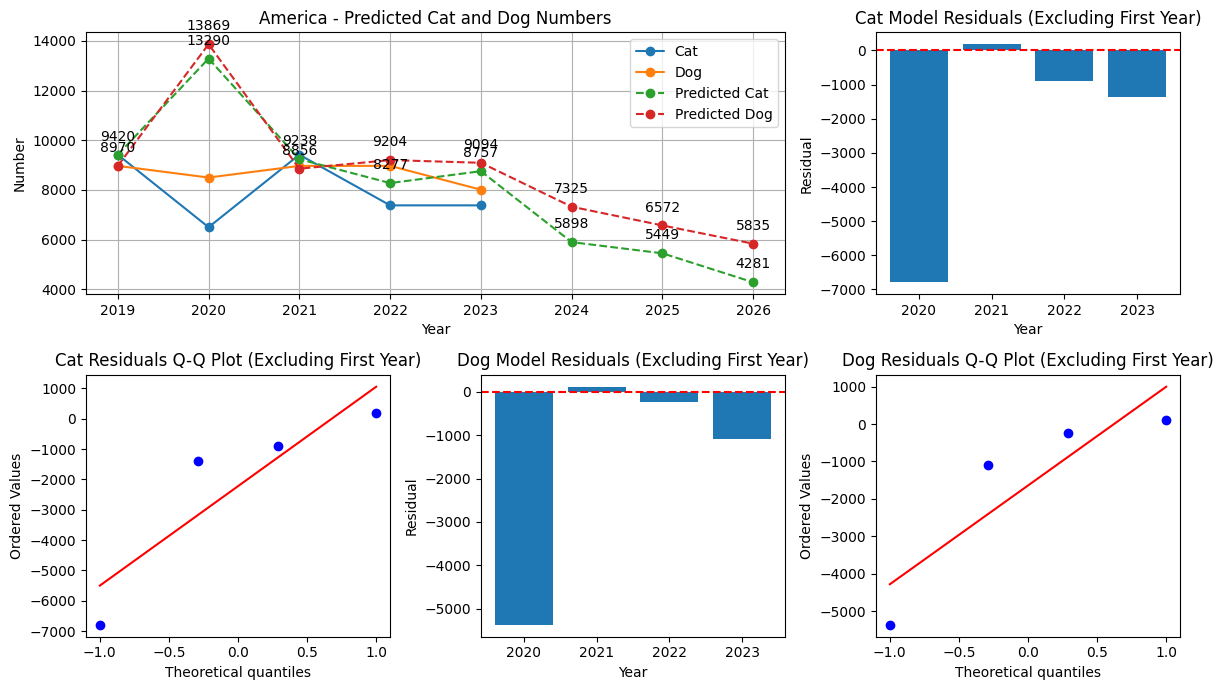
\includegraphics[width=.8\textwidth]{america_pets_forecast_k2.png}
	\caption{Predicted Cat and Dog Population in America (k=2)}
\end{figure}
\begin{table}[htbp]
\small % 缩小表格字体
\centering
\caption{MSE Evaluation Results}
\begin{tabular}{cccc}
\toprule
Differencing Order & Cat Model MSE & Dog Model MSE & Total MSE \\
\midrule
k=0 & 241270.72 & 60995.11 & 302265.84 \\
k=1 & 685887.84 & 264694.30 & 950582.15 \\
k=2 & 12211070.97 & 7516437.89 & 19727508.86 \\
\bottomrule
\end{tabular}
\end{table}
\par We can see that when \(k=0\), the fitting effect is the best.
So we get the predicted data with \(k=0\).
Up to now, we have got the predicted data of cat and dog population in China, America, France and Germany.
\subsubsection{Forecast food demand}
\begin{assumption}
    Most of the pets in the world are cats and dogs, so the demand for cat and dog food accounts for the majority of the total pet food demand.
\end{assumption}
\begin{assumption}
    Pet dogs are averaged as medium-sized dogs.
\end{assumption}
\par The average annual food demand for a medium-sized dog is 150 kg of dog food, and the average annual food demand for a cat is 40 kg of cat food.\cite{4}
\begin{assumption}
    China represents the 70 \% developing countries or Asian countries, France and Germany represent 40 \% Europe.
\end{assumption}
 \[demands=\sum_{i=1}^{k} count_i \times demand_{pet_i}\]
\par We can get the demand for pet food globally.(2019-2023 can be also calculated by the way in order to be used in the next question)

\begin{table}[htbp]
\centering
\caption{Global Pet Food Demand Forecast}
\begin{tabular}{cc}
\toprule
Year & Demand (kg) \\
\midrule
2019 & 3,657,480 \\
2020 & 3,510,655 \\
2021 & 3,889,390 \\
2022 & 3,788,490 \\
2023 & 3,640,150 \\
2024 & 3,982,670 \\
2025 & 3,735,530 \\
2026 & 3,995,310 \\
\bottomrule
\end{tabular}
\end{table}


\subsection{Question 3 Analysis}
\subsubsection{Convert units}
\par Note that the units are different, so we need to convert the units. First, convert USD to CNY.(Regard as 2024/11/23 because of ignoring the policy impact)\cite{5}
\[1USD=7.24CNY\]
\subsubsection{Remove 2019 data}
\par Additionally, we removed 2019 data, because it is too old and from 2020 to 2023, the data is smoother influenced by COVID-19.
It can better reflect the recovery process without the influence of 2019 data.
\subsubsection{Multiple linear regression model}
\par Using the similar method as the first question, we use the multiple linear regression model to fit the plane, and finally get the estimated value.
\par Considering the length of the article and the process is the same, here only the results are displayed.
\begin{figure}[htbp]
	\centering
	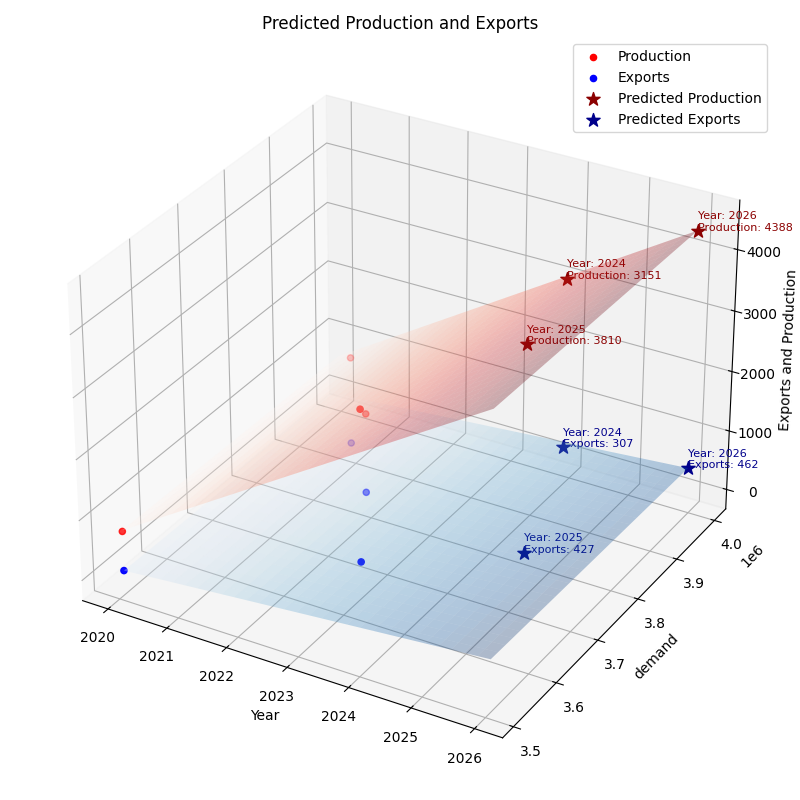
\includegraphics[width=.99\textwidth]{Figure_1111.png}
	\caption{Predicted Production and Exports}
\end{figure}
\begin{table}[htbp]
\centering
\caption{China's Pet Food Production and Export Forecast}
\begin{tabular}{ccc}
\toprule
Year & Production (CNY) & Export (CNY) \\
\midrule
2024 & 3151 & 307 \\
2025 & 3180 & 427 \\
2026 & 4388 & 462 \\
\bottomrule
\end{tabular}
\end{table}
\subsection{Question 4 Analysis}
\par The pet food industry in China will inevitably be affected by the new economic policies of European and American countries.
\subsubsection{Influence model}
\par We can use the influence model to analyze the impact of the new economic policies on the pet food industry in China.
\begin{definition}[impact]
    let \(I=impact\), \(J=judgment\), \(A=auxiliary\), \(\Delta J=\Delta judgment\), \(\Delta A=\Delta auxiliary\),
    \(P=production\), \(E=exports\), \(T=pets\_total\)
    \[J = P + 5 \times E + 0.01\times T\]
    \[A = America(T) + France(T) + Germany(T)\]
    \[\Delta J = J(year) - J(year-1)\]
    \[\Delta A = A(year) - A(year-1)\]
    \[I = 0.5 \times \Delta J - \Delta A\]
\end{definition}
\par \(\Delta A\) is the change of pets economy in America, France and Germany, which can be seen as the standard of the global pet economy's change.
\par \(\Delta J\) is the change of China's pet economy, and \(impact\) is the impact of the global pet economy on China's pet economy.
\(\Delta J\) is a mix of the standard change (\(\Delta A\)) and the actual change (\(\Delta J\)).
\par \(0.5\) is the weight of the change of China's pet economy and the global pet economy.
\par If \(I > 0\), it means that the global pet economy has a positive impact on China's pet economy, and vice versa.
Normally, the bigger the impact, the less negative the impact is.
\begin{figure}[htbp]
	\centering
	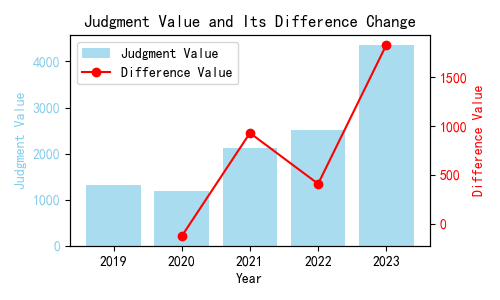
\includegraphics[width=.7\textwidth]{Figure_22.png}
	\caption{judgment value}
\end{figure}
\begin{figure}[htbp]
	\centering
	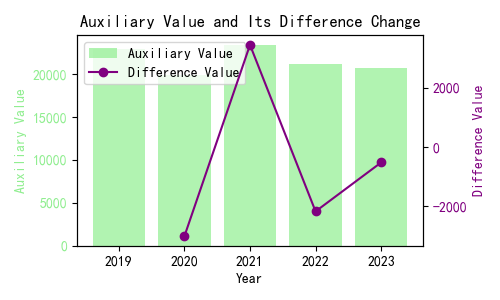
\includegraphics[width=.7\textwidth]{Figure_21.png}
	\caption{auxiliary value}
\end{figure}
\clearpage
\begin{figure}[htbp]
	\centering
	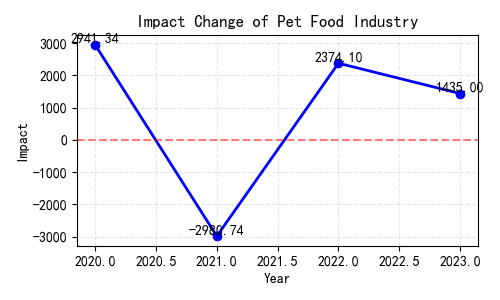
\includegraphics[width=.7\textwidth]{Figure_23.png}
	\caption{impact value}
\end{figure}

\subsubsection{Advice}
\par We can find that except for 2021, the development of China's pet food industry has always exceeded that of other Western countries.
But this does not mean that China has totally not been affected by the new economic policies of European and American countries.
The impact may probably be more positive in the future if the following advice is taken.
\begin{itemize}
    \item China should continue to increase the production of pet food to meet the increasing demand.
    \item China should also increase the export of pet food to other countries to reduce the impact of the new economic policies.
\end{itemize}

\section{Conclusion}
\par Combined all factors and data, we can conclude such information.
\begin{itemize}
    \item China's cats will increase a lot while dogs may stay nearly unchanged.
    \item The global demand for pet food will not change much.
    \item The production of pet food in China is far more than the export.
    \item The production of pet food will increase a lot while the export will not be witnessed big change.
    \item China should continue to expand pet food production to meet the growing demand and increase exports to other countries in order to mitigate the impact of the new economic policies.
\end{itemize}
\clearpage
\bibliography{books}



% \bigskip
% table环境是一个将表格嵌入文本的浮动环境。
% tabular环境的必选参数由每列对应一个格式字符所组成:c表示居中,l表示左对齐,r表示右对齐,其总
% 个数应与表的列数相同。此外,\verb|@{文本}|可以出现在任意两个上述的列格式之间,其中的文将被插入每一行
% 的同一位置。表格的各行以\verb|\\|分隔,同一行的各列则以\&分隔。
% \verb|\toprule|、\verb|\midrule|和\verb|\bottomrule|三个命令是由booktabs宏包提供的,其
% 中\verb|\toprule|和\verb|\bottomrule|分别用来绘制表格的第一条(表格最顶部)和第三条(表格最底部)水平线,
% \verb|\midrule|用来绘制第二条(表头之下)水平线,且第一条和第三条水平线的线宽为1.5pt,第二条水平线的线宽为1pt。
% 引用方法:“如表~\verb|\ref{标签名}|~所示”。


% %参考文献
% \begin{thebibliography}{9}%宽度9
%  \bibitem{bib:one} ....
%  \bibitem{bib:two} ....
% \end{thebibliography}

% \newpage
% %附录
% \begin{appendices}
% \section{排队算法--matlab 源程序}
% \begin{lstlisting}[language=matlab]
% kk=2;[mdd,ndd]=size(dd);
% while ~isempty(V)
% [tmpd,j]=min(W(i,V));tmpj=V(j);
% for k=2:ndd
% [tmp1,jj]=min(dd(1,k)+W(dd(2,k),V));
% tmp2=V(jj);tt(k-1,:)=[tmp1,tmp2,jj];
% end
% tmp=[tmpd,tmpj,j;tt];[tmp3,tmp4]=min(tmp(:,1));
% if tmp3==tmpd, ss(1:2,kk)=[i;tmp(tmp4,2)];
% else,tmp5=find(ss(:,tmp4)~=0);tmp6=length(tmp5);
% if dd(2,tmp4)==ss(tmp6,tmp4)
% ss(1:tmp6+1,kk)=[ss(tmp5,tmp4);tmp(tmp4,2)];
% else, ss(1:3,kk)=[i;dd(2,tmp4);tmp(tmp4,2)];
% end;end
% dd=[dd,[tmp3;tmp(tmp4,2)]];V(tmp(tmp4,3))=[];
% [mdd,ndd]=size(dd);kk=kk+1;
% end; S=ss; D=dd(1,:);
%  \end{lstlisting}
%  \section{规划解决程序--lingo源代码}
% \begin{lstlisting}[language=c]
% kk=2;
% [mdd,ndd]=size(dd);
% while ~isempty(V)
%     [tmpd,j]=min(W(i,V));tmpj=V(j);
% for k=2:ndd
%     [tmp1,jj]=min(dd(1,k)+W(dd(2,k),V));
%     tmp2=V(jj);tt(k-1,:)=[tmp1,tmp2,jj];
% end
%     tmp=[tmpd,tmpj,j;tt];[tmp3,tmp4]=min(tmp(:,1));
% if tmp3==tmpd, ss(1:2,kk)=[i;tmp(tmp4,2)];
% else,tmp5=find(ss(:,tmp4)~=0);tmp6=length(tmp5);
% if dd(2,tmp4)==ss(tmp6,tmp4)
%     ss(1:tmp6+1,kk)=[ss(tmp5,tmp4);tmp(tmp4,2)];
% else, ss(1:3,kk)=[i;dd(2,tmp4);tmp(tmp4,2)];
% end;
% end
%     dd=[dd,[tmp3;tmp(tmp4,2)]];V(tmp(tmp4,3))=[];
%     [mdd,ndd]=size(dd);
%     kk=kk+1;
% end;
% S=ss;
% D=dd(1,:);
%  \end{lstlisting}
% \end{appendices}

\end{document} 